% \documentclass[instructions]{uqthesis}
\documentclass[final]{uqthesis} 


%*************************************
% FOR YOUR FINAL THESIS
%*************************************

%IMPORTANT! 
%The default document class (above - line 1 & 2) for the template is \documentclass[instructions]{uqthesis} - this document class will show instructional material and examples relevant to the preliminary material in the compiled PDF preview. THESE INSTRUCTIONS ARE FOR YOUR REFERENCE ONLY AND ARE NOT TO BE INCLUDED IN YOUR FINAL THESIS! 

%To turn off these instructions in your final thesis you MUST use the document class \documentclass[final]{uqthesis} 
%To activate the final thesis document class you must UN-COMMENT THIS DOCUMENT CLASS (remove the % from the start of line 2) and comment out the instructional document class on line 1 (add % to the start of line 1). 

%*************************************
% Introduction to template
%*************************************
%This is The University of Queensland Graduate School Official LaTeX Thesis template.

%Be sure to observe the content of comments within the source code, these are prefaced with a percentage symbol.
%Most important instructions have been CAPITALISED.
%To uncomment an inactive command (if required) remove the % from in front of the command.

%Please see the README for more information.

%This file loads the necessary packages, sets the page styles, and defines required macros.
%Edit this if you are comfortable with LaTeX.

%Other tweaks can be made in uqthesis.cls, but change these at your own risk!

%See README for version.

%You must have the memoir class installed.

% ***************************************************
% LaTeX Packages
% ***************************************************
% This file defines the document design.
% Usually it is not necessary to edit this file, but you can use it to change aspects of the design if you want.

%There are essential packages that are contained within the uqthesis.cls which are integral to the template - These must not be deleted.  A list of these packages can be found in the README.tet file

%The packages below are optional, please add or alter as required.

% \usepackage{cite}				 %Allows abbreviated numerical citations.
\usepackage{pdfpages}			 %Allows you to include full-page pdfs.
\usepackage{wrapfig}			 %Lets you wrap text around figures.
\usepackage{bm} 				 %Bolded maths characters.
\usepackage{upgreek}			 %Upright Greek characters.
\usepackage{dsfont}				 %Double-struck fonts.
% \usepackage{simplewick}			 %For typesetting Wick contractions.
\usepackage{mathtools}		     %Can be used to fine-tune the maths presentation.	
\usepackage{framed}			     %For boxed text.
\usepackage{microtype}			 %pdfLaTeX will fix your kerning.
% \usepackage{marvosym}			 %Include symbols (like the Euro symbol, etc.).
% \usepackage{color}				 %Nice for scalable pdf graphics using InkScape.
% \usepackage{transparent}	     %Nice for scalable pdf graphics using InkScape.
% \usepackage{placeins}			 %Lets you put in a \FloatBarrier to stop figures floating past this command.
\usepackage{mdframed,mdwlist}    %Use these for nice lists (less white space).
\usepackage{graphicx}            %Enhanced support for graphics.
\usepackage{float}               %Improved interface for floating objects. 
% \usepackage{longtable}           %Allow tables to flow over page boundaries.
\usepackage{mathdots}            %Changed the basic LaTeX and plain TeX commands.
\usepackage{eucal}               %Font shape definitions to use the Euler script symbols in math mode.
\usepackage{array}               %Extending the array and tabular environments.
\usepackage{stmaryrd}            %The StMary’s Road symbol font.
\usepackage{amsthm}              %St Mary Road symbols for theoretical computer science. 
% \usepackage{pifont}              %Access to PostScript standard Symbol and Dingbats fonts.
% \usepackage{lipsum}              %Easy access to the Lorem Ipsum dummy text.
\usepackage{enumerate}           %Enumerate with redefinable labels. 
% \usepackage[all]{xy}             %This is a special package for drawing diagrams.
\usepackage{amsmath}             %ATypesetting theorems (AMS style).
\usepackage{amssymb}             %Provided an extended symbol collection.
\usepackage[utf8]{inputenc}      %Allowed all displayable utf8 characters to be available as input.
\usepackage{fancyhdr}            %Extensive control of page headers and footers.
% \usepackage{blindtext}           %Produced 'blind' text for testing.
% \usepackage{tikz}                %To create graphic elements.
% \usepackage[figuresright]{rotating}	%Allows large tables to be rotated to landscape.
% \usetikzlibrary{shapes.geometric, arrows}
%You can add more packages here if you need

%This defines some macros that implement Latin abbreviations
%COMMENT OUT OR DELETE IF UNDESIRED.
% \newcommand{\via}{\textit{via}} %Italicised via.
% \newcommand{\ie}{\textit{i.e.}} %Literally.
% \newcommand{\eg}{\textit{e.g.}} %For example.
% \newcommand{\etc}{\textit{etc.}} %So on...
% \newcommand{\vv}{\textit{vice versa}} %And the other way around.
% \newcommand{\viz}{\textit{viz}.} %Resulting in.
% \newcommand{\cf}{\textit{cf}.} %See, or 'consistent with'.
% \newcommand{\apr}{\textit{a priori}} %Before the fact.
% \newcommand{\apo}{\textit{a posteriori}} %After the fact.
% \newcommand{\vivo}{\textit{in vivo}} %In the flesh.
% \newcommand{\situ}{\textit{in situ}} %On location.
% \newcommand{\silico}{\textit{in silico}} %Simulation.
% \newcommand{\vitro}{\textit{in vitro}} %In glass.
% \newcommand{\vs}{\textit{versus}} %James \vs{} Pete.
% \newcommand{\ala}{\textit{\`{a} la}} %In the manner of...
% \newcommand{\apriori}{\textit{a priori}} %Before hand.
% \newcommand{\etal}{\textit{et al.}} %And others, with correct punctuation.
% \newcommand{\naive}{na\"\i{}ve} %Queen Amidala is young and \naive{}.

% ***************************************************
% Title page
% ***************************************************
%***THESIS TITLE***
%Use Sentence Case (capitalise only the first word and proper nouns).
\title{Title here: Subtitle}

%***YOUR NAME***
%Do not include initials or middle names. Do not include your supervisor(s)' name(s).
\author{Candidate's full name}
%***YOUR CURRENT DEGREES***
%Use abbreviations. Do not include the date or location of your degree. Do not include the degree for which this thesis is being submitted.
\currentdegrees{Candidate’s academic degrees}

%***ORCID ID***
%Add and hyperlink your ORCID
\orcid{\href{add your ORCID url here}{Candidate's ORCID}}

%***YEAR OF SUBMISSION***
\date{Year}
%***TYPE OF DEGREE***
\submittedfor{Doctor}
%If this thesis is being submitted for Masters, comment out the above line (add % before line) and remove comment (by removing %) from line below
%\submittedfor{Masters}

%***YOUR SCHOOL***
%Use Title Case (capitalise every word which is not a conjunction or preposition).
%See - http://blog.apastyle.org/apastyle/2012/03/title-case-and-sentence-case-capitalization-in-apa-style.html - for help.
\school{Name of the Enrolling Unit}

\begin{document}

\frontmatter
% Assemble title page
\maketitle
\clearpage

% ***************************************************
% Preface
%****************************************************
\section{Abstract}
\normalfont
%Open abstract.tex to edit
% ***************************************************
% Abstract
% ***************************************************
% TO PRODUCE A STAND-ALONE PDF OF YOUR ABSTRACT, uncomment this section and the \end{document} at the end of the file by removing the % from the start of each line.

%\documentclass[12pt, a4paper]{memoir}

%% ***************************************************
% LaTeX Packages
% ***************************************************
% This file defines the document design.
% Usually it is not necessary to edit this file, but you can use it to change aspects of the design if you want.

%There are essential packages that are contained within the uqthesis.cls which are integral to the template - These must not be deleted.  A list of these packages can be found in the README.tet file

%The packages below are optional, please add or alter as required.

% \usepackage{cite}				 %Allows abbreviated numerical citations.
\usepackage{pdfpages}			 %Allows you to include full-page pdfs.
\usepackage{wrapfig}			 %Lets you wrap text around figures.
\usepackage{bm} 				 %Bolded maths characters.
\usepackage{upgreek}			 %Upright Greek characters.
\usepackage{dsfont}				 %Double-struck fonts.
% \usepackage{simplewick}			 %For typesetting Wick contractions.
\usepackage{mathtools}		     %Can be used to fine-tune the maths presentation.	
\usepackage{framed}			     %For boxed text.
\usepackage{microtype}			 %pdfLaTeX will fix your kerning.
% \usepackage{marvosym}			 %Include symbols (like the Euro symbol, etc.).
% \usepackage{color}				 %Nice for scalable pdf graphics using InkScape.
% \usepackage{transparent}	     %Nice for scalable pdf graphics using InkScape.
% \usepackage{placeins}			 %Lets you put in a \FloatBarrier to stop figures floating past this command.
\usepackage{mdframed,mdwlist}    %Use these for nice lists (less white space).
\usepackage{graphicx}            %Enhanced support for graphics.
\usepackage{float}               %Improved interface for floating objects. 
% \usepackage{longtable}           %Allow tables to flow over page boundaries.
\usepackage{mathdots}            %Changed the basic LaTeX and plain TeX commands.
\usepackage{eucal}               %Font shape definitions to use the Euler script symbols in math mode.
\usepackage{array}               %Extending the array and tabular environments.
\usepackage{stmaryrd}            %The StMary’s Road symbol font.
\usepackage{amsthm}              %St Mary Road symbols for theoretical computer science. 
% \usepackage{pifont}              %Access to PostScript standard Symbol and Dingbats fonts.
% \usepackage{lipsum}              %Easy access to the Lorem Ipsum dummy text.
\usepackage{enumerate}           %Enumerate with redefinable labels. 
% \usepackage[all]{xy}             %This is a special package for drawing diagrams.
\usepackage{amsmath}             %ATypesetting theorems (AMS style).
\usepackage{amssymb}             %Provided an extended symbol collection.
\usepackage[utf8]{inputenc}      %Allowed all displayable utf8 characters to be available as input.
\usepackage{fancyhdr}            %Extensive control of page headers and footers.
% \usepackage{blindtext}           %Produced 'blind' text for testing.
% \usepackage{tikz}                %To create graphic elements.
% \usepackage[figuresright]{rotating}	%Allows large tables to be rotated to landscape.
% \usetikzlibrary{shapes.geometric, arrows}
%You can add more packages here if you need

%This defines some macros that implement Latin abbreviations
%COMMENT OUT OR DELETE IF UNDESIRED.
% \newcommand{\via}{\textit{via}} %Italicised via.
% \newcommand{\ie}{\textit{i.e.}} %Literally.
% \newcommand{\eg}{\textit{e.g.}} %For example.
% \newcommand{\etc}{\textit{etc.}} %So on...
% \newcommand{\vv}{\textit{vice versa}} %And the other way around.
% \newcommand{\viz}{\textit{viz}.} %Resulting in.
% \newcommand{\cf}{\textit{cf}.} %See, or 'consistent with'.
% \newcommand{\apr}{\textit{a priori}} %Before the fact.
% \newcommand{\apo}{\textit{a posteriori}} %After the fact.
% \newcommand{\vivo}{\textit{in vivo}} %In the flesh.
% \newcommand{\situ}{\textit{in situ}} %On location.
% \newcommand{\silico}{\textit{in silico}} %Simulation.
% \newcommand{\vitro}{\textit{in vitro}} %In glass.
% \newcommand{\vs}{\textit{versus}} %James \vs{} Pete.
% \newcommand{\ala}{\textit{\`{a} la}} %In the manner of...
% \newcommand{\apriori}{\textit{a priori}} %Before hand.
% \newcommand{\etal}{\textit{et al.}} %And others, with correct punctuation.
% \newcommand{\naive}{na\"\i{}ve} %Queen Amidala is young and \naive{}.

%\begin{document}

%\begin{center}
	%\textbf{\large Your title goes here}

	%\textbf{Abstract}

	%Your Name, The University of Queensland, 20??
%\end{center}

% ********* Enter your text below this line: ********
Start this section on a new page [this template will automatically handle this]. \\

\noindent
The abstract should outline the main approach and findings of the thesis and normally must be between 300 and 800 words.

% ***************************************************

%\end{document}

\clearpage
% ***************************************************
\section*{Declaration by author}
%DO NOT EDIT.
% ***************************************************
% Declaration by Author
% ***************************************************
% This is the DECLARATION BY AUTHOR
% All candidates to reproduce this section in their thesis verbatim
% DO NOT EDIT!
%
\begin{instructional}
\textit{(All candidates to reproduce this section in their thesis verbatim)\\}
\end{instructional}

\noindent
This thesis is composed of my original work, and contains no material previously published or written by another person except where due reference has been made in the text. I have clearly stated the contribution by others to jointly-authored works that I have included in my thesis.\\

\noindent
I have clearly stated the contribution of others to my thesis as a whole, including statistical assistance, survey design, data analysis, significant technical procedures, professional editorial advice, financial support and any other original research work used or reported in my thesis. The content of my thesis is the result of work I have carried out since the commencement of my higher degree by research candidature and does not include a substantial part of work that has been submitted to qualify for the award of any other degree or diploma in any university or other tertiary institution. I have clearly stated which parts of my thesis, if any, have been submitted to qualify for another award.\\

\noindent
I acknowledge that an electronic copy of my thesis must be lodged with the University Library and, subject to the policy and procedures of The University of Queensland, the thesis be made available for research and study in accordance with the Copyright Act 1968 unless a period of embargo has been approved by the Dean of the Graduate School. \\

\noindent
I acknowledge that copyright of all material contained in my thesis resides with the copyright holder(s) of that material. Where appropriate I have obtained copyright permission from the copyright holder to reproduce material in this thesis and have sought permission from co-authors for any jointly authored works included in the thesis.

\clearpage
%YOU MUST EDIT THIS DOCUMENT.
% ***************************************************
% PRELIMINARY PAGES
% ***************************************************
% The instructions contained within this part of the thesis template need to be suppressed from the final thesis. There are instructions on how to do this in the MainThesis.tex file.

% To ensure your work is not suppressed with the instructions please add your text only where instructed.


%***Publications included in this thesis***
\section*{Publications included in this thesis}

\begin{instructional}

	Start this section on a new page [this template will automatically handle this].\\
	
	\noindent
	If you choose to include publications as part of your thesis as described in UQ policy (\href{http://ppl.app.uq.edu.au/content/4.60.07-alternate-thesis-format-options}{\color{blue}{PPL 4.60.07 Alternative Thesis Format Options}}) use this section to detail accepted or in press publication/s using the standard citation format for your discipline. \\
    
    \noindent
	Papers submitted for publication and awaiting review should appear in the next section, \textbf{Submitted manuscripts included in this thesis}.\\
    
    \noindent
	On the page immediately preceding the chapter that includes your publication, in no more than one (1) page, describe your contribution to the authorship if you are not a sole author. In describing your contribution, you must satisfy the University's authorship policy (\href{http://ppl.app.uq.edu.au/content/4.20.04-authorship}{\color{blue}{PPL 4.20.04 Authorship}}). Authorship is based on having made a substantive contribution to at least one, and usually more than one, of the following activities:
	%
	\begin{enumerate}
		\item	conception and design of the project;
		\item	analysis and interpretation of the research data on which the publication is based;
		\item	drafting significant parts of the publication or critically reviewing it so as to contribute to the interpretation.
	\end{enumerate}
	
	\noindent
	As an author, you must have participated sufficiently in the publication to take public responsibility for at least that part of the work that you contributed.\\
    
    \noindent
	It may be useful to refer to specific parts of the methods, analyses, results, or discussion to illustrate your contribution to the paper.\\
    
    \noindent
	If you have not included any of your publications in the thesis then state ``No publications included''.\\
	
	\textbf{Example:}
	\begin{enumerate}

    \item \cite{DumyCitationKey} \textbf{Your Name}, Co-author 1, and Final Author, \href{linktoyourpaper}{Title of your paper}, \textit{Journal}, Issue, Number, Year

    \item \cite{DumyCitationKey} \textbf{Your Name}, Co-author 1, and Final Author, \href{linktoyourpaper}{Title of your paper}, \textit{Journal}, Issue, Number, Year

    \end{enumerate}
	
\end{instructional}

% ********* Enter your text below this line: ********


% ***************************************************


%***Submitted manuscripts included in this thesis***
\section*{Submitted manuscripts included in this thesis}

\begin{instructional}
	List manuscript/s submitted for publication here. As described above for \textbf{Publications included in the thesis}, on the page immediately preceding the chapter that includes the submitted manuscript, in no more than one (1) page, detail your contribution to the authorship if you are not the sole author.\\
    
    \noindent
    If you have no submitted manuscripts from your candidature then state ``No manuscripts submitted for publication''.\\
    
    \textbf{Example:}
    \begin{enumerate}

    \item \cite{DumyCitationKey} \textbf{Your Name}, Co-author 1, and Final Author, Title of your paper, submitted to \textit{Journal} on 4th June 2018.

    \end{enumerate}
\end{instructional}

% ********* Enter your text below this line: ********


% ***************************************************


%***Other publications during candidature***
\section*{Other publications during candidature}

\begin{instructional}
    List other publications arising during your candidature using the standard citation format for your discipline. Divide your publications into sub-sections as appropriate in your discipline \eg{} peer-reviewed papers, book chapters, conference abstracts. Papers submitted for publication and awaiting review are not considered publications and cannot be included in this section.\\
    
    \noindent
    If you have no publications from your candidature then state ``No other publications''.\\
    
    \textbf{Example:}
    \subsection*{Conference abstracts}

    \begin{enumerate}

    \item \cite{DumyCitationKey} \textbf{Your Name}, Co-author 1, and Final Author, Title of your conference paper, \textit{Proceedings of Conference}, other details.

    \end{enumerate}

    \subsection*{Book chapters}

    \begin{enumerate}

    \item \cite{DumyCitationKey} \textbf{Your Name}, Co-author 1, and Final Author, Title of your chapter, Book, editor, \etc{}.

    \end{enumerate}

\end{instructional}

% ********* Enter your text below this line: ********


% ***************************************************


%***Contributions by others to the thesis***
\section*{Contributions by others to the thesis}

\begin{instructional}
	List the significant and substantial inputs made by others to the research, work and writing represented and/or reported in the thesis. These could include significant contributions to: the conception and design of the project; non-routine technical work; analysis and interpretation of research data; drafting significant parts of the work or critically revising it so as to contribute to the interpretation. \\
    
    \noindent
	If no one contributed significantly then state ``No contributions by others''.
\end{instructional}

% ********* Enter your text below this line: ********


% ***************************************************


%***Statement of parts of the thesis submitted to qualify for the award of another degree***
\section*{Statement of parts of the thesis submitted to qualify for the award of another degree}

\begin{instructional}
    The thesis must be comprised only of research undertaken while enrolled in the HDR program unless otherwise approved by the Dean, Graduate School in advance of submission.\\
    
    \noindent
    If you have been given permission to include your previous work that has been used towards another degree, you must list the relevant parts of the thesis that incorporates this work including, the degree name, year and institution, and the outcome of the submission of material. \\
    
    \noindent
    If no parts of the thesis have been submitted in this way then state ``No works submitted towards another degree have been included in this thesis''.
\end{instructional}

% ********* Enter your text below this line: ********


% ***************************************************


%***Research involving human or animal subjects***
\section*{Research involving human or animal subjects}

\begin{instructional}
	All research involving human or animal subjects requires prior ethical review and approval by an independent review committee. At UQ, the relevant committee for research involving human subjects is the \href{http://www.uq.edu.au/research/integrity-compliance/human-ethics}{\color{blue}{Human Ethics Unit}} and the relevant committee for research involving animal subjects is the relevant \href{http://www.uq.edu.au/research/integrity-compliance/animal-welfare}{\color{blue}{Animal Ethics Committee}}.  Please provide details of any ethics approvals obtained including the ethics approval number and name of approving committees.  A copy of the ethics approval letter must be included in the thesis appendix.\\
    
    \noindent
	If no human or animal subjects were involved in this research please state: ``No animal or human subjects were involved in this research''.
\end{instructional}

% ********* Enter your text below this line: ********


% ***************************************************


%***Acknowledgements***
\clearpage
\section*{Acknowledgments}

\begin{instructional}
    Start this section on a new page [the template will handle this for you].\\
    
    \noindent
    Acknowledgements recognise those who have been instrumental in the completion of the project.  Acknowledgements should include any professional editorial advice received including the name of the editor and a brief description of the service rendered.
\end{instructional}

% ********* Enter your text below this line: ********


% ***************************************************


%***Financial Support***
\clearpage
\section*{Financial support}

\begin{instructional}
    Start this section on a new page [the template will handle this for you].\\
    
    \noindent
    If you are the recipient of an Australian Government Research Training Program (RTP) scholarship, you are required to acknowledge this contribution.  Please include the text below:\\
    
    \noindent
    ``This research was supported by an Australian Government Research Training Program Scholarship''\\
    
    \noindent
    If you received any other financial support for your project, you are also required to acknowledge the funding body/bodies in this section.\\
    
    \noindent
    If no financial provided then state ``No financial support was provided to fund this research''.
\end{instructional}

% ********* Enter your text below this line: ********


% ***************************************************


%***Keywords***
\section*{Keywords}

\begin{instructional}
	Maximum 10 words; use lower case throughout, separating words/phrases with commas. For example: word, word word, word, word, word word
\end{instructional}
% ********* Enter your text below this line: ********


% ***************************************************


%***Australian and New Zealand Standard Research Classifications (ANZSRC)***
\section*{Australian and New Zealand Standard Research Classifications (ANZSRC)}

\begin{instructional}
    Provide data that links your thesis to the disciplines and discipline clusters in the Federal Government’s Excellence in Research for Australia (ERA) initiative.\\
    
    \noindent
    Please allocate the thesis a \textbf{maximum of 3} \href{http://www.abs.gov.au/Ausstats/abs@.nsf/Latestproducts/6BB427AB9696C225CA2574180004463E?opendocument}{\color{blue}{Australian and New Zealand Standard Research Classifications (ANZSRC) codes}} at the \textbf{6 digit level} and include the descriptor and a percent weighting for each code. Total percent must add to 100.\\


\textbf{Example:}\\


    ANZSRC code: 060101, Analytical Biochemistry, 60\% \\
    \indent ANZSRC code: 060104, Cell Metabolism, 20\% \\
    \indent ANZSRC code: 060199, Biochemistry and Cell Biology not elsewhere classified, 20\%
\end{instructional}

% ********* Enter your text below this line: ********


% ***************************************************


%***Fields of Research (FoR) Classification***
\section*{Fields of Research (FoR) Classification}

\begin{instructional}
    Allows for categorisation of the thesis according to the field of research. \\
    
    \noindent
    Please allocate the thesis a \textbf{maximum of 3} \href{http://www.abs.gov.au/Ausstats/abs@.nsf/Latestproducts/6BB427AB9696C225CA2574180004463E?opendocument}{\color{blue}{Fields of Research (FoR) Codes}} at the \textbf{4 digit level} and include the descriptor and a percent weighting for each code. Total percent must add to 100. \\

\textbf{Example:}\\

FoR code: 0601, Biochemistry and Cell Biology, 80\% \\
\indent FoR code: 0699, Other Biological Sciences, 20\%
\end{instructional}

% ********* Enter your text below this line: ********


% ***************************************************


%***Order of remaining thesis content***
\begin{instructional}
\section*{Order for the Remainder of the Thesis}
\noindent
    Remainder of the thesis should be in the following order

    \begin{itemize}
        \item Dedications (if applicable)
        \item Table of Contents
        \item List of Figures and Tables
        \item List of Abbreviations used in the thesis
        \item Main text of the thesis
        \item Bibliography or List of References
        \item Appendices
    \end{itemize}

\noindent
\textbf{Date of thesis template release:} 22 March 2019
\end{instructional}
\clearpage


%***Dedication***
%If you wish to add a dedication (if appropriate), do so here.
%If not, comment out from here...
	\rmfamily
	\normalfont

	\begin{vplace}[1]
		\begin{center}
			This template is dedicated to nerds everywhere.
		\end{center}
	\end{vplace}

%... to here.

\clearpage
\pagestyle{headings}


%***Table of Contents***
%These generate the table of contents, list of figures, and list of tables from items tagged with a \label{} command.
\tableofcontents
	\clearpage
\listoffigures
	\clearpage
\listoftables
\newpage
%*************************************
% List of abbreviations
%*************************************
% You can make a list of abbreviations here.
%
% There are LaTeX packages available to take care of these things, but you will
% need to manually add these to the template at this stage (support may be added
% in future releases).

%CHOOSE AN APPROPRIATE TITLE.
%\chapter[List of abbreviations]{List of abbreviations}
\chapter[List of Abbreviations and Symbols]{List of Abbreviations and Symbols}

%If the auto-sizing of the tables annoys you, consider the tabularx package.

%List of abbreviations.
\begin{center}
	\small
	\begin{longtable}{ll}
	\toprule
	Abbreviations & {} \\
	\bottomrule
	AC				& Alternating Current \\
	AFM				& Atomic Force Microscopy/Microscope \\
	\etc{}		&	\etc{} \\
	\hline
	\end{longtable}
\end{center}

%*************************************
% List of symbols
%*************************************
%List of symbols. REMOVE IF NOT NEEDED.
\begin{center}
	\small
	\begin{longtable}{ll}
	\toprule
	Symbols & {} \\
	\bottomrule
	$\hat{\rho}$		& Density operator \\
	\etc{}					& \etc{} \\
	\hline
	\end{longtable}
\end{center}

%***End of list of symbols and abbreviations*** %List of symbols. REMOVE IF NOT NEEDED.

%***End of front matter***

% ***************************************************
% Thesis Content
%****************************************************
\mainmatter

%Each chapter is a separate .tex file. Use \input to load them here, as demonstrated below for Chapter 1 and Chapter 2.
%We recommend keeping each in a separate subfolder, with its accompanying figures, etc. This is how the template is currently structured.
%If you wish to divide your thesis into parts (each containing multiple chapters), us the \part{} command.

%CHAPTER 1
\chapter[Introduction]{Introduction}
\label{Chap:Intro}

% ***************************************************
% Introduction
% ***************************************************

\section{Your thesis topic}
%Replace "Your thesis topic" with what will become the \label{} for this section.

% ********* Enter your text below this line: ********
Introduce your topic.

% ***************************************************

%CHAPTER 2
%If you are presenting work which has been previously published, acknowledge this here.
% ***************************************************
% How to introduce a previously published chapter
% ***************************************************
%This is an example of how you might introduce a chapter that has been published previously. 
\cleartoevenpage
\pagestyle{empty}	
%Use this command (above) to suppress the header from the preceding chapter.

\noindent
The following publication has been incorporated as Chapter~\ref{Chap:label}.

\noindent
1.~\cite{DumyCitationKey} \textbf{Your Name}, Co-author 1, and Final Author, \href{linktoyourpaper}{Title of your paper}, \textit{Journal} Issue, Number, Year

\begin{table}[h]
	\begin{center}
	\begin{tabular}{|c|l|l|}
		\hline
		Contributor & Statement of contribution & \% \\
		\hline
		\textbf{Your Name}				& writing of text 					& 70\\
															& proof-reading							& 60 \\
															& theoretical derivations 	& 70\\
															& numerical calculations 		& 100\\
															& preparation of figures 		& 80 \\
															& initial concept						& 10 \\
		\hline
		Co-author 1								& writing of text 					& 20\\
															& proof-reading							& 10 \\
															& supervision, guidance 		& 20\\
															& theoretical derivations 	& 10\\
															& preparation of figures 		& 20 \\
															& initial concept						& 10 \\
		\hline
		Final Author							& writing of text 					& 10\\
															& proof-reading							& 30 \\
															& supervision, guidance 		& 80 \\
															& theoretical derivations 	& 20 \\
															& preparation of figures 		& 10 \\
															& initial concept						& 80 \\
		\hline
	\end{tabular}
	\end{center}
\end{table}

If your task breakdown requires further clarification, do so here. Do not exceed a single page.


% ***************************************************
% Example of an internal chapter
% ***************************************************
%This is an internal chapter of the thesis.
%If you have a long title, you can supply an abbreviated version to print in the Table of Contents using the optional argument to the \chapter command.
\chapter[Abbreviated title]{Full title}
\label{Chap:label}	%CREATE YOUR OWN LABEL.
\pagestyle{headings}

% ********* Enter your text below this line: ********
Introduce the broad layout of the chapter.

% ***************************************************


\section{Introduction}
\label{Sec:label}	%CREATE YOUR OWN LABEL.

% ********* Enter your text below this line: ********
Add your text here. 

% ***************************************************


% HOW TO ADD ADDITIONAL CHAPTERS
% Step One: Add a new folder called "ChapterX" (X being the chapter number).
% Step Two: Within the folder add a new .tex file by clicking the "New File" button in the Overleaf Menu. Rename the file to a title of your choice.
% Step Three: Copy the Chapter 2 headline and "\input" command located above and insert it below Chapter 2.
% Step Four: Rename the headline to your specific chapter number, change the input command to include the name of the folder you created and the name of the file you created.
% Repeat this process for every chapter.

%CONCLUSION CHAPTER
% ***************************************************
% Conclusion
% ***************************************************
\chapter[Conclusion]{Conclusion}
\label{Chap:Conclusion}

% ********* Enter your text below this line: ********
Conclude your thesis.

% ***************************************************

% ***************************************************
% Bibliography
%****************************************************
%CHOOSE YOUR BIB STYLE AND FILE.
%We have included the following two referencing styles for you to use in your thesis. You can add an alternate style if you prefer.

%Style: apalike = this is an (Author, Year) referencing style similar to APA
%Style: elsarticle-num = this is a numbered referencing style that will display the bibliography in citation order

%To use one of the styles provided ensure the % is removed from the start of the line, and the other option is commented out with a % at the start of the line. The style elsarticle-num is active by default.

%\bibliographystyle{apalike}
\bibliographystyle{elsarticle-num}

\bibliography{./References/Bibliography}

%When you have finished your thesis we recommend that you manually fix any errors in your bibliography. 
%To do this, compile, copy the .bbl into a new .tex file and include this here after commenting out the other bibliography commands. Make corrections in that .tex file.

% ***************************************************
% Appendices
%**************************************************** 
%UNCOMMENT THIS SECTION IF YOU ARE USING APPENDICES.
%Simply adapt the same formatting used for other chapters.
\appendix
% If you need appendix in your thesis then consider the following appendix file (you can add more if you need more) otherwise you should not consider it in your main thesis.
% ***************************************************
% Appendix
% ***************************************************
\chapter{Appendix}

Write your appendix here. Following two are examples. 


\section{Name of Appendix-1}


\section{Name of Appendix-2}





% ***************************************************
% Examples
%**************************************************** 
% The following files are only for examples and you should not include them in your final thesis.
% ***************************************************
% Example of Citations
% ***************************************************
%This example is provided for your reference only. DO NOT INCLUDE IN YOUR FINAL THESIS. 
\chapter{Example of Citations}

This text is only for Bibliography testing purposes. This is a book by Cawvey et al.~\cite{Cawvey2017}. There are few journal articles~\cite{Pakzad2018, Adachi2007} in this bibliography. This is a proceeding paper~\cite{J.Fenwick2010}.  This is a PhD thesis by Peerling~\cite{PeerlingPhD1999}. These are few other types of citations~\cite{Panis2004}.
% ***************************************************
% Example of Code; how to import Code in pdf.
% ***************************************************
%This example is provided for your reference only. DO NOT INCLUDE IN YOUR FINAL THESIS. 
\chapter{Example of Code}

\section{Find the greatest number from a list of numbers in \textit{Python}}

\begin{verbatim}

a=[1,2,3,4,6,7,99,88,999]
    max= 0
    for i in a:
        if i > max:
            max=i
    print(max)

\end{verbatim}
% ***************************************************
% Example of Equations
% ***************************************************
%This example is provided for your reference only. DO NOT INCLUDE IN YOUR FINAL THESIS. 
\chapter{Example of Equations}

\begin{equation}
    E = mc^2
\end{equation}


\begin{align}
    a = {}& b + c\\
    x = {}& y + z
\end{align}


\begin{equation}
    \begin{split}
        a = {}& b + c\\
            {}& + d + e
    \end{split} 
\nonumber
\end{equation}
    
    
\begin{equation} 
sinx+cosx=1 
\end{equation}



% ***************************************************
% Example of Figures
% ***************************************************
%This example is provided for your reference only. DO NOT INCLUDE IN YOUR FINAL THESIS. 

%\begin{figure} : If you put no command after \begin{table} then this figure will be printed anywhere in your pdf where LaTex finds the free space to put it. If you wish to specify where the figure goes you have to give a command in LaTex after  \begin{figure}. 
%
%There are different commands to put the figure in different positions e.g. \begin{table}[h] LaTex will print the figure in the same position that you put it in your source file, if there is enough space to print it
%N.B. it is important to note that commanding LaTeX to add a figure in a specific place may result in formatting issues.

\chapter{Example of Figures}

\begin{figure}[h]
\begin{center}
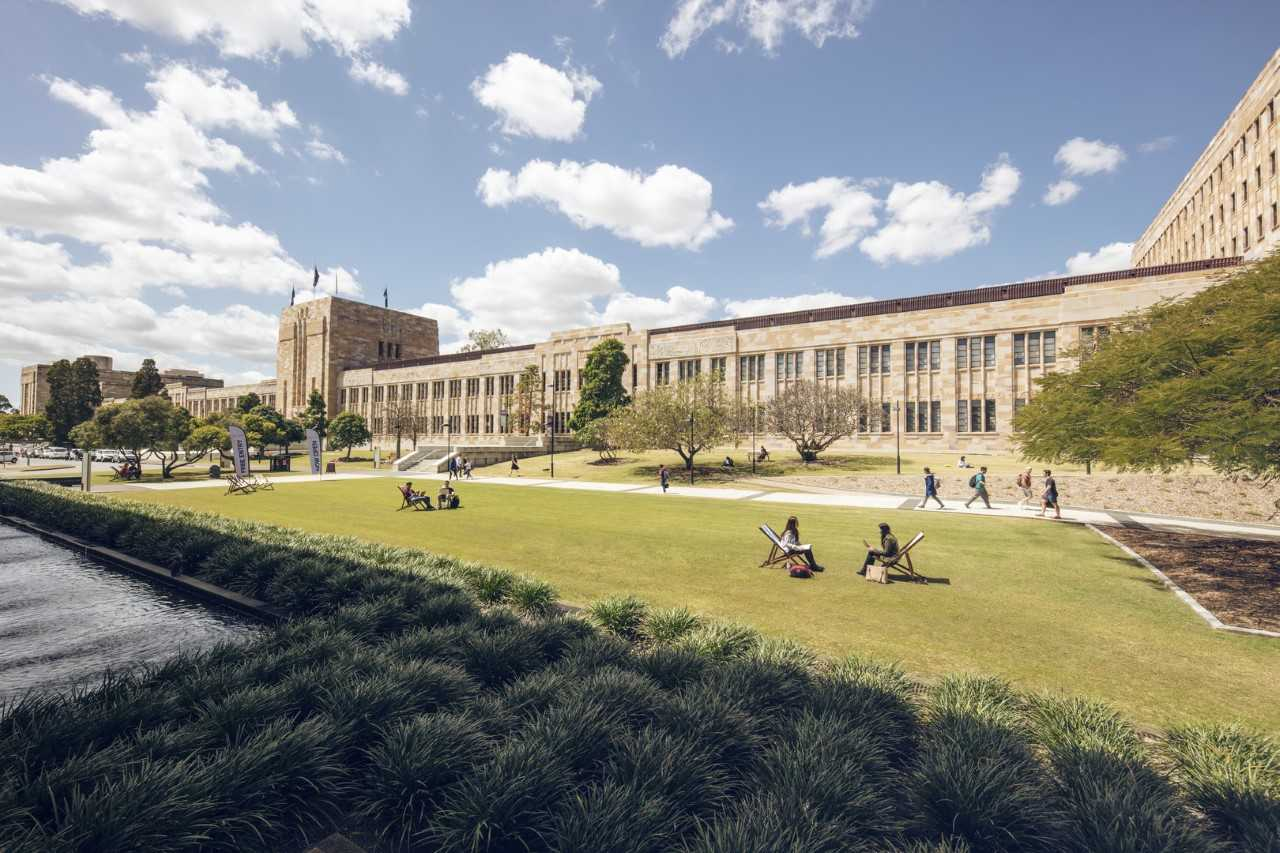
\includegraphics[width=1.0\textwidth]{Examples/FigureUQ}
\caption{The University Of Queensland}
\label{Fig:1}
\end{center}
\end{figure}

The Figure~\ref{Fig:1} represents beauty of the UQ campus.
% ***************************************************
% Example of Flow Charts
% ***************************************************
%This example is provided for your reference only. DO NOT INCLUDE IN YOUR FINAL THESIS. 
\chapter{Example of Flow Charts}
\begin{figure}[h]
\caption{Flow Chart}
\label{Fig:FlowChart}
\begin{center}
\tikzstyle{decision} = [diamond, draw, fill=white!10, 
    text width=4.5em, text badly centered, node distance=3cm, inner sep=0pt]
\tikzstyle{block} = [rectangle, draw, fill=white!20, 
    text width=5em, text centered, rounded corners, minimum height=4em]
\tikzstyle{line} = [draw, -latex']
\tikzstyle{cloud} = [draw, ellipse,fill=white!20, node distance=3cm,
    minimum height=2em]
    
\begin{tikzpicture}[node distance = 2cm, auto]
    % Place nodes
    \node [block] (Step1) {initialize model};
    \node [cloud, left of=Step1] (expert) {expert};
    \node [cloud, right of=Step1] (system) {system};
    \node [block, below of=Step1] (identify) {identify candidate models};
    \node [block, below of=identify] (evaluate) {evaluate candidate models};
    \node [block, left of=evaluate, node distance=3cm] (update) {update model};
    \node [decision, below of=evaluate] (decide) {is best candidate better?};
    \node [block, below of=decide, node distance=3cm] (stop) {stop};
    % Draw edges
    \path [line] (Step1) -- (identify);
    \path [line] (identify) -- (evaluate);
    \path [line] (evaluate) -- (decide);
    \path [line] (decide) -| node [near start] {yes} (update);
    \path [line] (update) |- (identify);
    \path [line] (decide) -- node {no}(stop);
    \path [line,dashed] (expert) -- (Step1);
    \path [line,dashed] (system) -- (Step1);
    \path [line,dashed] (system) |- (evaluate);
\end{tikzpicture}
\end{center}
\end{figure}

Flow chart~\ref{Fig:FlowChart} is a simple example.
% ***************************************************
% Example of Tables
% ***************************************************
%This example is provided for your reference only. DO NOT INCLUDE IN YOUR FINAL THESIS. 
\chapter{Example of Tables}

Here is a really simple table~\ref{Table}.


%\begin{table} : If you put no command after \begin{table} then this table will be printed anywhere in your pdf where LaTex finds the free space to put it. If you wish to specify where the table goes you have to give a command in LaTex after  \begin{table}. 
%
%There are different commands to put the table in different positions e.g. \begin{table}[h] LaTex will print the table in the same position that you put it in your source file, if there is enough space to print it
%N.B. it is important to note that commanding LaTeX to add a table in a specific place may result in formatting issues.

\begin{table}[h]
\caption{Name of the Australian Cities}
\begin{center}
\begin{tabular}{{|c|c|c|}}
\hline
\textbf{Number}& \textbf {Name}\\
\hline
      1& Brisbane\\
      2& Sydney\\
      3& Melbourne\\
      4& Canberra\\
      5& Perth\\
      6& Adelaide\\
      7& Hobart\\
      8& Darwin\\
\hline
\end{tabular}
\end{center}
\label{Table}
\end{table}


% ***************************************************
% Back Matter
%**************************************************** 
%COMMENT OUT IF YOU DO NOT WISH TO INCLUDE BACK MATTER.
% ***************************************************
% Back Matter
% ***************************************************
% ADD AN ENDQUOTE HERE. If you do not wish to, delete this file.
\backmatter

\normalfont
\cleartooddpage

\pagestyle{empty}

\begin{table}[b!]
\begin{center}
% ********* Enter your quote within {} brackets: ********
\textit{Endquote goes here.}

% ********************************************************
\end{center}
\begin{flushright}
% ********* Enter your text below, as indicated: ********
Author of quote,\\
Source of quote

% ********************************************************
\end{flushright}
\end{table}

\end{document}
